% Options for packages loaded elsewhere
\PassOptionsToPackage{unicode}{hyperref}
\PassOptionsToPackage{hyphens}{url}
\PassOptionsToPackage{dvipsnames,svgnames,x11names}{xcolor}
%
\documentclass[
  letterpaper,
  DIV=11,
  numbers=noendperiod]{scrreprt}

\usepackage{amsmath,amssymb}
\usepackage{iftex}
\ifPDFTeX
  \usepackage[T1]{fontenc}
  \usepackage[utf8]{inputenc}
  \usepackage{textcomp} % provide euro and other symbols
\else % if luatex or xetex
  \usepackage{unicode-math}
  \defaultfontfeatures{Scale=MatchLowercase}
  \defaultfontfeatures[\rmfamily]{Ligatures=TeX,Scale=1}
\fi
\usepackage{lmodern}
\ifPDFTeX\else  
    % xetex/luatex font selection
\fi
% Use upquote if available, for straight quotes in verbatim environments
\IfFileExists{upquote.sty}{\usepackage{upquote}}{}
\IfFileExists{microtype.sty}{% use microtype if available
  \usepackage[]{microtype}
  \UseMicrotypeSet[protrusion]{basicmath} % disable protrusion for tt fonts
}{}
\makeatletter
\@ifundefined{KOMAClassName}{% if non-KOMA class
  \IfFileExists{parskip.sty}{%
    \usepackage{parskip}
  }{% else
    \setlength{\parindent}{0pt}
    \setlength{\parskip}{6pt plus 2pt minus 1pt}}
}{% if KOMA class
  \KOMAoptions{parskip=half}}
\makeatother
\usepackage{xcolor}
\setlength{\emergencystretch}{3em} % prevent overfull lines
\setcounter{secnumdepth}{2}
% Make \paragraph and \subparagraph free-standing
\ifx\paragraph\undefined\else
  \let\oldparagraph\paragraph
  \renewcommand{\paragraph}[1]{\oldparagraph{#1}\mbox{}}
\fi
\ifx\subparagraph\undefined\else
  \let\oldsubparagraph\subparagraph
  \renewcommand{\subparagraph}[1]{\oldsubparagraph{#1}\mbox{}}
\fi


\providecommand{\tightlist}{%
  \setlength{\itemsep}{0pt}\setlength{\parskip}{0pt}}\usepackage{longtable,booktabs,array}
\usepackage{calc} % for calculating minipage widths
% Correct order of tables after \paragraph or \subparagraph
\usepackage{etoolbox}
\makeatletter
\patchcmd\longtable{\par}{\if@noskipsec\mbox{}\fi\par}{}{}
\makeatother
% Allow footnotes in longtable head/foot
\IfFileExists{footnotehyper.sty}{\usepackage{footnotehyper}}{\usepackage{footnote}}
\makesavenoteenv{longtable}
\usepackage{graphicx}
\makeatletter
\def\maxwidth{\ifdim\Gin@nat@width>\linewidth\linewidth\else\Gin@nat@width\fi}
\def\maxheight{\ifdim\Gin@nat@height>\textheight\textheight\else\Gin@nat@height\fi}
\makeatother
% Scale images if necessary, so that they will not overflow the page
% margins by default, and it is still possible to overwrite the defaults
% using explicit options in \includegraphics[width, height, ...]{}
\setkeys{Gin}{width=\maxwidth,height=\maxheight,keepaspectratio}
% Set default figure placement to htbp
\makeatletter
\def\fps@figure{htbp}
\makeatother
\newlength{\cslhangindent}
\setlength{\cslhangindent}{1.5em}
\newlength{\csllabelwidth}
\setlength{\csllabelwidth}{3em}
\newlength{\cslentryspacingunit} % times entry-spacing
\setlength{\cslentryspacingunit}{\parskip}
\newenvironment{CSLReferences}[2] % #1 hanging-ident, #2 entry spacing
 {% don't indent paragraphs
  \setlength{\parindent}{0pt}
  % turn on hanging indent if param 1 is 1
  \ifodd #1
  \let\oldpar\par
  \def\par{\hangindent=\cslhangindent\oldpar}
  \fi
  % set entry spacing
  \setlength{\parskip}{#2\cslentryspacingunit}
 }%
 {}
\usepackage{calc}
\newcommand{\CSLBlock}[1]{#1\hfill\break}
\newcommand{\CSLLeftMargin}[1]{\parbox[t]{\csllabelwidth}{#1}}
\newcommand{\CSLRightInline}[1]{\parbox[t]{\linewidth - \csllabelwidth}{#1}\break}
\newcommand{\CSLIndent}[1]{\hspace{\cslhangindent}#1}

\KOMAoption{captions}{tableheading}
\makeatletter
\makeatother
\makeatletter
\@ifpackageloaded{bookmark}{}{\usepackage{bookmark}}
\makeatother
\makeatletter
\@ifpackageloaded{caption}{}{\usepackage{caption}}
\AtBeginDocument{%
\ifdefined\contentsname
  \renewcommand*\contentsname{Table of contents}
\else
  \newcommand\contentsname{Table of contents}
\fi
\ifdefined\listfigurename
  \renewcommand*\listfigurename{List of Figures}
\else
  \newcommand\listfigurename{List of Figures}
\fi
\ifdefined\listtablename
  \renewcommand*\listtablename{List of Tables}
\else
  \newcommand\listtablename{List of Tables}
\fi
\ifdefined\figurename
  \renewcommand*\figurename{Figure}
\else
  \newcommand\figurename{Figure}
\fi
\ifdefined\tablename
  \renewcommand*\tablename{Table}
\else
  \newcommand\tablename{Table}
\fi
}
\@ifpackageloaded{float}{}{\usepackage{float}}
\floatstyle{ruled}
\@ifundefined{c@chapter}{\newfloat{codelisting}{h}{lop}}{\newfloat{codelisting}{h}{lop}[chapter]}
\floatname{codelisting}{Listing}
\newcommand*\listoflistings{\listof{codelisting}{List of Listings}}
\makeatother
\makeatletter
\@ifpackageloaded{caption}{}{\usepackage{caption}}
\@ifpackageloaded{subcaption}{}{\usepackage{subcaption}}
\makeatother
\makeatletter
\@ifpackageloaded{tcolorbox}{}{\usepackage[skins,breakable]{tcolorbox}}
\makeatother
\makeatletter
\@ifundefined{shadecolor}{\definecolor{shadecolor}{rgb}{.97, .97, .97}}
\makeatother
\makeatletter
\makeatother
\makeatletter
\makeatother
\ifLuaTeX
  \usepackage{selnolig}  % disable illegal ligatures
\fi
\IfFileExists{bookmark.sty}{\usepackage{bookmark}}{\usepackage{hyperref}}
\IfFileExists{xurl.sty}{\usepackage{xurl}}{} % add URL line breaks if available
\urlstyle{same} % disable monospaced font for URLs
\hypersetup{
  pdftitle={Hierarchical Spatial Structure in Compartmental Epidemiological models},
  pdfauthor={James Bender},
  colorlinks=true,
  linkcolor={blue},
  filecolor={Maroon},
  citecolor={Blue},
  urlcolor={Blue},
  pdfcreator={LaTeX via pandoc}}

\title{Hierarchical Spatial Structure in Compartmental Epidemiological
models}
\author{James Bender}
\date{}

\begin{document}
\maketitle
\ifdefined\Shaded\renewenvironment{Shaded}{\begin{tcolorbox}[boxrule=0pt, frame hidden, sharp corners, borderline west={3pt}{0pt}{shadecolor}, breakable, interior hidden, enhanced]}{\end{tcolorbox}}\fi

\renewcommand*\contentsname{Sections}
{
\hypersetup{linkcolor=}
\setcounter{tocdepth}{2}
\tableofcontents
}
\bookmarksetup{startatroot}

\hypertarget{copyright-notice}{%
\chapter*{Copyright notice}\label{copyright-notice}}
\addcontentsline{toc}{chapter}{Copyright notice}

\markboth{Copyright notice}{Copyright notice}

© Susan Su (2023).

\begin{quote}
Delete following statement if not relevant.
\end{quote}

I certify that I have made all reasonable efforts to secure copyright
permissions for third-party content included in this thesis and have not
knowingly added copyright content to my work without the owner's
permission.

\bookmarksetup{startatroot}

\hypertarget{abstract}{%
\chapter*{Abstract}\label{abstract}}
\addcontentsline{toc}{chapter}{Abstract}

\markboth{Abstract}{Abstract}

Epidemiological modelling is essential to understand and predict the
spread of infectious diseases and plan effective interventions. Disease
spread is an inherently spatial process, particularly in diseases that
spread through contact with body fluids, and spatially structured
epidemiological models provide an opportunity to incorporate a wealth of
geographical information into the modelling process. Here, we present a
compartmental meta-population model encoding the hierarchical spatial
structure of the Australian Statistical Geography Standard (ASGS).
Relationships between spatial groupings are represented in a mixing
matrix, which influences the spread of infection between patches
(i.e.~Patches in the same spatial grouping are more likely to spread
disease to each other compared to patches outside this grouping). As an
example, we model the Greater Melbourne Statistical Area (SA) with
patches representing SA2, SA4, and SA4 level groupings, and
stochastically simulate the course of an epidemic as a Continuous Time
Markov Chain (CTMC). We compare the results of simulations with varying
influence of the spatial relationships between patches (through the
construction of the mixing matrix), different levels of spatial
resolution (which level of the spatial hierarchy is represented by
compartmental patches), and different infectious disease parameters
(e.g.~\(R_0\)), as well as with the results of a spatial compartmental
model incorporating an alternative source of geographic information
(i.e.~empirically derived mobility data). We conclude by speculating on
the potential use of such geographically informed epidemiological models
in the management of infectious diseases.

\bookmarksetup{startatroot}

\hypertarget{declaration}{%
\chapter*{Declaration}\label{declaration}}
\addcontentsline{toc}{chapter}{Declaration}

\markboth{Declaration}{Declaration}

\begin{quote}
Use only one of the following declarations.
\end{quote}

\hypertarget{standard-thesis}{%
\section*{Standard thesis}\label{standard-thesis}}
\addcontentsline{toc}{section}{Standard thesis}

\markright{Standard thesis}

This thesis is an original work of my research and contains no material
which has been accepted for the award of any other degree or diploma at
any university or equivalent institution and that, to the best of my
knowledge and belief, this thesis contains no material previously
published or written by another person, except where due reference is
made in the text of the thesis.

Student name:

Student signature:

Date:

\hypertarget{publications-during-enrolment}{%
\subsection*{Publications during
enrolment}\label{publications-during-enrolment}}
\addcontentsline{toc}{subsection}{Publications during enrolment}

\begin{quote}
Remove this section if you do not have publications.
\end{quote}

The material in sec-intro has been submitted to the journal
\emph{Journal of Impossible Results} for possible publication.

The contribution in sec-litreview of this thesis was presented in the
International Symposium on Nonsense held in Dublin, Ireland, in July
2022.

\hypertarget{reproducibility-statement}{%
\subsection*{Reproducibility
statement}\label{reproducibility-statement}}
\addcontentsline{toc}{subsection}{Reproducibility statement}

This thesis is written using Quarto with renv (Ushey, 2022) to create a
reproducible environment. All materials (including the data sets and
source files) required to reproduce this document can be found at the
Github repository
\href{https://github.com/SusanSu/thesis}{\texttt{github.com/SusanSu/thesis}}.

This work is licensed under a
\href{http://creativecommons.org/licenses/by-nc-sa/4.0/}{Creative
Commons Attribution-NonCommercial-ShareAlike 4.0 International License}.

\hypertarget{thesis-including-published-works-declaration}{%
\section*{Thesis including published works
declaration}\label{thesis-including-published-works-declaration}}
\addcontentsline{toc}{section}{Thesis including published works
declaration}

\markright{Thesis including published works declaration}

I hereby declare that this thesis contains no material which has been
accepted for the award of any other degree or diploma at any university
or equivalent institution and that, to the best of my knowledge and
belief, this thesis contains no material previously published or written
by another person, except where due reference is made in the text of the
thesis.

This thesis includes ?? original papers published in peer reviewed
journals and ?? submitted publications. The ideas, development and
writing up of all the papers in the thesis were the principal
responsibility of myself, the student, working within the Department of
Econometrics \& Business Statistics under the supervision of ??

(The inclusion of co-authors reflects the fact that the work came from
active collaboration between researchers and acknowledges input into
team-based research.)

In the case of (??insert chapter numbers) my contribution to the work
involved the following:

I have / have not renumbered sections of submitted or published papers
in order to generate a consistent presentation within the thesis.

Student name:

Student signature:

Date:

I hereby certify that the above declaration correctly reflects the
nature and extent of the student's and co-authors' contributions to this
work. In instances where I am not the responsible author I have
consulted with the responsible author to agree on the respective
contributions of the authors.

Main Supervisor name:

Main Supervisor signature:

Date:

\bookmarksetup{startatroot}

\hypertarget{acknowledgements}{%
\chapter*{Acknowledgements}\label{acknowledgements}}
\addcontentsline{toc}{chapter}{Acknowledgements}

\markboth{Acknowledgements}{Acknowledgements}

I would like to thank my pet goldfish for \ldots{}

\begin{quote}
In accordance with Chapter 7.1.4 of the research degrees handbook, if
you have engaged the services of a~professional~editor, you
must~provide~their name~and a brief description of the service rendered.
If the professional editor's current or former area of academic
specialisation is similar your own, this too should be stated as it may
suggest to examiners that the editor's advice to the student has
extended beyond guidance on English expression to affect the substance
and structure of the thesis.
\end{quote}

\begin{quote}
Free text section for you to record your acknowledgment and gratitude
for the more general academic input and support such as financial
support from grants and scholarships and the non-academic support you
have received during the course of your enrolment. If you are a
recipient of the ``Australian Government Research Training Program
Scholarship'', you are required to include the following statement:
\end{quote}

\begin{quote}
\begin{quote}
``This research was supported by an Australian Government Research
Training Program (RTP) Scholarship.''
\end{quote}
\end{quote}

\begin{quote}
You may also wish to acknowledge significant and substantial
contribution made by others to the research, work and writing
represented and/or reported in the thesis. These could include
significant contributions to: the conception and design of the project;
non-routine technical work; analysis and interpretation of research
data; drafting significant parts of the work or critically revising it
so as to contribute to the interpretation.
\end{quote}

\clearpage\pagenumbering{arabic}\setcounter{page}{0}

\bookmarksetup{startatroot}

\hypertarget{sec-intro}{%
\chapter{Introduction \& Background}\label{sec-intro}}

\hypertarget{modelling-infectious-epidemics}{%
\section{Modelling Infectious
Epidemics}\label{modelling-infectious-epidemics}}

``Epidemic models are used to inform decisions on disease prevention,
surveillance, control and treatment and can be applied to new
epidemics'' (\textbf{bjørnstad2020?})

\hypertarget{compartment-models}{%
\section{Compartment Models}\label{compartment-models}}

``Compartmental models are the most frequently used type of epidemic
model. In this class of models, individuals can be in a finite number of
discrete states. Some of these states are simply labels that specify the
various traits of individuals. Of these, some will be changing with
time, such as age class, and others will be fixed, such as sex or
species. Other states indicate the progress of an infection: for
example, an individual can upon becoming infected, typically first enter
a state of latency, then progress to a state of infectiousness, and then
lose infected status to progress to a recovered/immune state. With each
state one can associate the subpopulation of individuals who are in that
particular state at the given time (e.g.~a female in a latent state of
infection). Often the same symbol is used as a label for a state and to
denote the corresponding subpopulation size, either as a fraction or as
a number (e.g.~I or Y for individuals in an infectious state)'' -
(\textbf{diekmann2010?})

\hypertarget{the-sir-compartmental-model}{%
\subsection{The SIR compartmental
model}\label{the-sir-compartmental-model}}

The simplest comparmental model of infectious disease spread is the SIR
Compartmental Model, with three compartments: S - for individuals
\emph{susceptible} to the disease; I - for \emph{infected} individuals;
and R - for previously infected individuals who have \emph{recovered}
(or been otherwise \emph{removed} from that compartment). With the
simplifying assumption of a constant population size, \(N\), i.e.

\begin{equation}\protect\hypertarget{eq-SIR_N}{}{
N = S + I + R
}\label{eq-SIR_N}\end{equation}

Individuals move between compartments in a fixed set of ways, they may
either become infected (moving from S -\textgreater{} I), or recover
from infection (I -\textgreater{} R).

At each time unit an infected individual can come into contact with, on
average, \(k\frac{S}{N}\) Susceptible individuals. \(\pi\) is the
probability of infecting somebody on coming in contact, so
\(\beta = k\pi\) is the average rate at which an infected indivudual
will infect a susceptible. Infected individuals recover at the constant
rate, \(\gamma\), with \(1/\gamma\) the mean recovery time.

\begin{longtable}[]{@{}ll@{}}
\toprule\noalign{}
Parameter & Interpretation \\
\midrule\noalign{}
\endhead
\bottomrule\noalign{}
\endlastfoot
\(\beta\) & Transmission rate \\
\(\gamma\) & Recovery rate \\
\end{longtable}

Thus, an SIR model can be represented by the schematic

\hypertarget{sir-dynamics}{%
\section{SIR Dynamics}\label{sir-dynamics}}

\hypertarget{ode-representation}{%
\subsection{ODE representation}\label{ode-representation}}

Given the rate parameters defined above, the change in compartment
composition over time can be described by the system of differential
equations

\begin{equation}\protect\hypertarget{eq-SIR-ODE}{}{
\begin{aligned}
& \frac{d S}{d t}=-\beta I \frac{S}{N} \\
& \frac{d I}{d t}=\beta I \frac{S}{N}-\gamma I \\
& \frac{d R}{d t}=\gamma I
\end{aligned}
}\label{eq-SIR-ODE}\end{equation} Importantly, if the total population
size is known, given Equation~\ref{eq-SIR_N}, R = N - S + I and the
entire system can be described by two of the equations in
Equation~\ref{eq-SIR-ODE}.

EXAMPLE

\hypertarget{limitations-of-deterministic-ode}{%
\subsubsection{Limitations of Deterministic
ODE}\label{limitations-of-deterministic-ode}}

While Equation~\ref{eq-SIR-ODE} provides a neat solution for the
expected behaviour of a epidemic, it fails to caputure the variability
inherent in a complex process like disease spread.

\hypertarget{stochastic-process-markov-chain-representation}{%
\subsection{Stochastic Process (Markov Chain)
Representation}\label{stochastic-process-markov-chain-representation}}

A Stochastic Process is a collection of random variables, \(X_t\).

\hypertarget{markov-chains}{%
\subsubsection{Markov chains}\label{markov-chains}}

A Markov chain is a sequence of random variables \(X_0, X_1, \ldots\)
taking values in \(S\) with the property that

\begin{equation}\protect\hypertarget{eq-Markov-Property}{}{
\begin{aligned}
P\left(X_{n+1}\right. & \left.=j \mid X_0=x_0, \ldots, X_{n-1}=x_{n-1}, X_n=i\right) \\
& =P\left(X_{n+1}=j \mid X_n=i\right),
\end{aligned}
}\label{eq-Markov-Property}\end{equation}

for all \(x_0, \ldots, x_{n-1}, i, j \in S\), and \(n \geq 0\). That is,
the state at the next time step is determined only by the state at the
current time step.

\hypertarget{time-homogeneity}{%
\subsubsection{Time Homogeneity}\label{time-homogeneity}}

While not a general property of Markov chains, all of those considered
in this work will have the additional property of \emph{time
homogeneity}:

\[
P\left(X_{n+1}=j \mid X_n=i\right)=P\left(X_1=j \mid X_0=i\right),
\] i.e.~the probabilities in Equation~\ref{eq-Markov-Property} do not
vary with \(t\)

\hypertarget{sir-dtmc}{%
\subsubsection{SIR DTMC}\label{sir-dtmc}}

An SIR Compartment model an be described by a Markov chain of two
independent random variables S(t) and I(t) representing the number of
susceptible or individuals infected at time t respectively (as in the
ODE case, a third RV R(t) denoting the number of recovered individuals
is fully determined when the population size is known, and can be left
out from this characterisation).

There are two potential events (tbl-SIR\_Events) resulting in a change
of state i.e.~from \(X_{t}\) to \(X_{t+\delta t}\)

\begin{equation}\protect\hypertarget{eq-SIR_DTMC_Trans}{}{
p _ {(s +k, i +j),(s,i)}(\Delta t) =
\begin{cases}
{\frac { \beta i s} { N}} \Delta t, & {(k, j) = (-1, 1) } \\ 
{ \gamma i \Delta t}, & { (k, j) = (0, -1)  } \\ 
{ 1 - \bigg[ \frac { \beta i s } { N } +  \gamma i }\bigg] \Delta t, & { (k, j) = (0, 0)} \\
0 & {otherwise}
\end{cases}
}\label{eq-SIR_DTMC_Trans}\end{equation}

\hypertarget{transition-matrix}{%
\paragraph{Transition Matrix}\label{transition-matrix}}

\hypertarget{sir-ctmc}{%
\subsubsection{SIR CTMC}\label{sir-ctmc}}

\bookmarksetup{startatroot}

\hypertarget{sec-MPMspec}{%
\chapter{Spatial Metapopulation Model}\label{sec-MPMspec}}

\hypertarget{specification}{%
\subsection{Specification}\label{specification}}

We employ a basic \(SIR\) compartmental model, assuming no births and
deaths, with a total of \(N\) individuals.
\begin{equation}\protect\hypertarget{eq-ConstantTotalPopulation}{}{ S + I  + R = N}\label{eq-ConstantTotalPopulation}\end{equation}

We divide the population into \(n\) connected sub-populations,hereafter
`patches', with \(N_i\) denoting the population of patch \(i\) (note
that \(N = \sum\limits_{i=1}^{n}N_i\)).

Let \(S_i\), \(I_i\), \(R_i\) respectively denote the number of
susceptible, infected and recovered individuals in Patch \(i\) (noting
also that \(N_i = S_i + I_i + R_i\)). Also, since
\(R_i = N_i - S_i - I_i\), we will not explicitly show \(R_i\) in the
equations hereafter (thought this could be calculated at any time)

Individuals coming into contact with an infective, whether within or
without patch, become infected at a rate \(\beta\).

While individuals do not migrate between patches, infectives from patch
\(i\) infect - individuals from \(j\) with a proportion \(\phi_{ij}\).

The force of infection in patch \(i\) given by \[
\Lambda_i = \beta \sum\limits_{j}^{n}\phi_{ij}I_j
\]

And thus the force of infection vector
\begin{equation}\protect\hypertarget{eq-FOIv}{}{\Lambda = \beta I \Phi}\label{eq-FOIv}\end{equation}

Where \(I\) is the vector of patch infection counts, and \(\Phi\) is the
mixing matrix.

\hypertarget{construction-of-mixing-matrix}{%
\subsection{Construction of mixing
matrix}\label{construction-of-mixing-matrix}}

Instead of constructing the mixing matrix from empirical OD data, we
specified the matrix analytically to encode the hierarchical structure
of the SA classification.

The main constraint employed was that patches within the same level
\(L\) SA region would mix together more strongly than those not.
Nevertheless, because of a higher level enclosing group (in the case of
Melbourne, the state level grouping), we only need to specify a series
of coefficients which correspond to the lowest level grouping in which
two patches co-occur. Furthermore, to ensure the matrix rows sum to one,
mixing is also proportional to the fraction of the population of the
grouping region comprised by the patch.

for any two patches \(i\) and \(j\),

\(i, j\) are patches

\(S_{i}^{L}\) is the set of patches in level \(L\) \(N_i\) is the
population of \(i\) \(N_{i}^{L}\) is the population of \(S_{i}^{L}\)
\(\xi^{L}(\delta)\) is the proportion of mixing that occurs within
\(S_{i}^{L}\) but not\(S_{i}^{L-1}\)

The intra level mixing coefficients \(\xi_L\) comprise the vector
\(\xi\). Constraining the elements of \(\xi\) s.t.
\(\sum\limits_{L = 1}^{L} \xi_i = 1\) (where \(L\) is the highest level
grouping) ensures the rows of the mixing matrix sum to unity.\\

-More verbosity

-Be more explicit about SA Levels

-Mention Mixing with PPMM

\hypertarget{implementation}{%
\subsection{Implementation}\label{implementation}}

The model was implemented as continuous time markov chain, with discrete
state variables \[S_{i}(t), I_{i}(t) \in {0,1,2,...N_{i}}\] where
\(t\in [0, \infty)\)

at \(t = 0\), a randomly selected patch, \(i\), is seeded with
\(I = 10\) invectives, such that
\[S_{i}(0) = N_{i} - 10, I_{i}(0) = 10\] and the remaining patches are
disease free \[S_j(0) = N_j, I_j(0) =0, i\neq j \]

at \(t>0\) possible changes in state (`events') are infection at a patch
\(i\) (if \(S_i \geq 1\) \& \(I \geq 1\)), or recovery at patch \(i\)
(if \(I_i \geq 1\)). Rates for these events are given in
Table~\ref{tbl-EventRates}

\hypertarget{tbl-EventRates}{}
\begin{longtable}[]{@{}lll@{}}
\caption{\label{tbl-EventRates}Event Rates}\tabularnewline
\toprule\noalign{}
Event & State change & Rate \\
\midrule\noalign{}
\endfirsthead
\toprule\noalign{}
Event & State change & Rate \\
\midrule\noalign{}
\endhead
\bottomrule\noalign{}
\endlastfoot
Infection in patch \(i\) & \(\{S_i -1, I_i +1\}\) & \(S_i \Lambda_i\) \\
Recovery in patch \(i\) & \(\{I_i - 1\}\) & \(\gamma I_i\) \\
\end{longtable}

Due to the Markov property, events occur after a exponentially
distributed time with parameter equal to the sum of all event rates
\[\Delta t \sim Exp(\lambda)\] where

\(\lambda = \sum\limits_{i}^{n}S_i \Lambda_i + \gamma I_i\)

at \(t + \delta t\), a random event from Table~\ref{tbl-EventRates} will
occur with probability directly proportional to it's rate.

When the system enters a disease free equilibrium state
(i.e.~\(I = 0\)), the implementation is complete.

\hypertarget{sec-MossGmelb}{%
\section{Example: Greater Melbourne Area Spatial Metapopulation
model}\label{sec-MossGmelb}}

\bookmarksetup{startatroot}

\hypertarget{sec-intro}{%
\chapter{Metapopulation Spatial resolution}\label{sec-intro}}

In Section~\ref{sec-MossGmelb}, we observed the construction of a
meta-population mixing matrix from empirical origin-destination (OD)
data. The patches used in the example were based on the `SA3' regions of
the Australian Statistical Geography Standard's Statistical Areas (SA)
classification (Australian Statistical Geography Standard (ASGS), 2023)
(comprising forty patches for the Greater Melbourne area in that
example).

\hypertarget{hierarchical-structure-of-the-sa-classification}{%
\section{Hierarchical Structure of the SA
classification}\label{hierarchical-structure-of-the-sa-classification}}

An important feature of the SA classification structure is that there
are multiples scale of classification and that lower levels of SA are
hierarchically nested within higher levels. For example, several SA3
regions are contained within a single SA4 region, and multiple SA4
regions are contained within the Greater Melbourne Capital City SA
(GMCCSA). Moreover, each SA3 region is partitioned into a number of SA2
scale regions (in the case of he GMCCSA, 361 of them), which in turn are
divided further into (for GMCCSA, 20xx) SA1 scale regions.
Figure~\ref{fig-GMelbSA2SA3SA4} shows the SA2, SA3, and SA4 regions of
the GMCCSA.

\begin{figure}

\begin{minipage}[t]{0.50\linewidth}

{\centering 

\raisebox{-\height}{

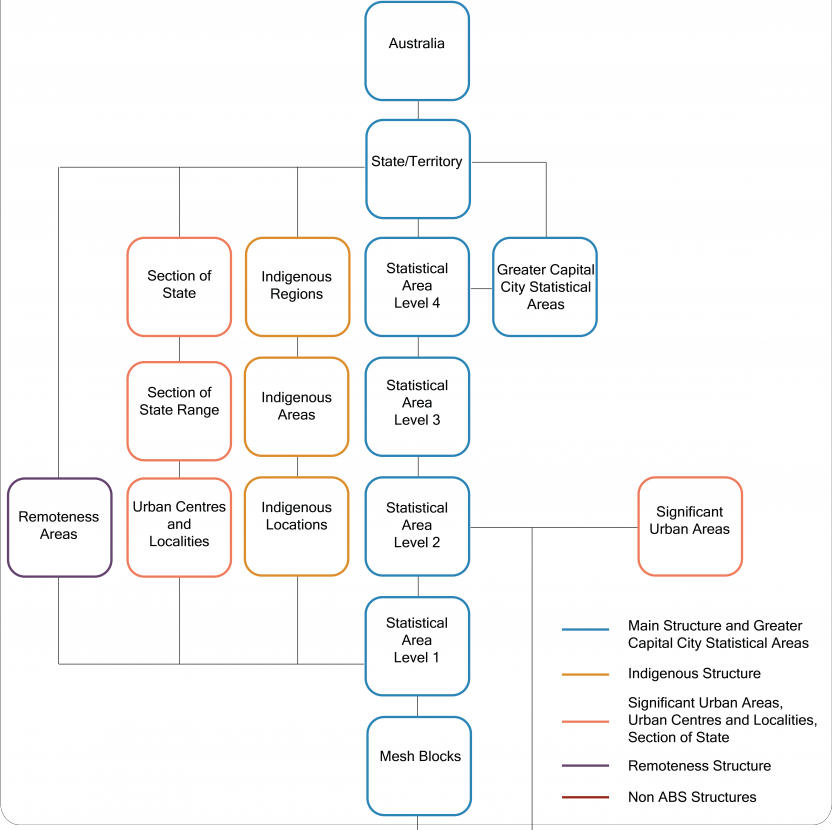
\includegraphics[width=4.83333in,height=\textheight]{ASGS_Diagram_2021.png}

}

}

\subcaption{\label{fig-ASGS}}
\end{minipage}%
%
\begin{minipage}[t]{0.50\linewidth}

{\centering 

\begin{figure}

{\centering 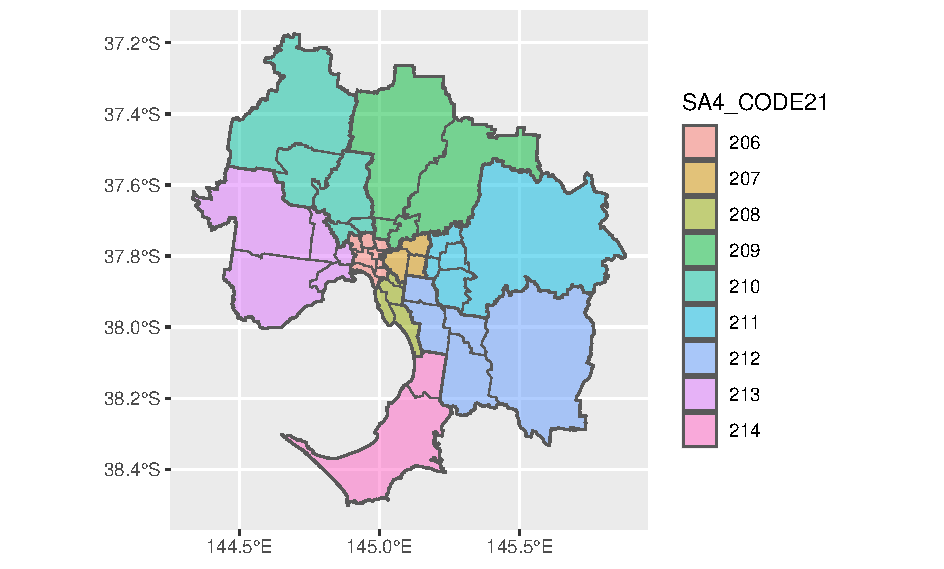
\includegraphics{03-CurrentStudy_files/figure-pdf/fig-GMelbSA2SA3SA4-1.pdf}

}

\end{figure}

}

\end{minipage}%

\caption{\label{fig-ASGSSA}Showing (a) the abstract structureof The
Australian Statistical Geography Standard (ASGS) Statistical Areas (SA)
Classification and (b) an example of SA3 and SA4 regions within the
Greater Melbourne Greater Capital City Statistical Area (GMGCCSA)}

\end{figure}

For specific example, the Maribyrnong (SA3) region sits inside the West
Melbourne (SA4) region alongside Essendon (SA3)
Figure~\ref{fig-FootscraySAexample}. Both West Melbourne and the
neighbouring `Inner Melbourne' (SA4), containing the city center and
other SA3 regions, are part of the GSCCSA. Moreover, within Marybirnong
(SA3) there are six SA2 level regions (Braybrook, Footscray,
Maribyrnong, Seddon - Kingsville, West Footscray - Tottenham,
Yarraville), which can likewise be partitioned in to smaller SA1 level
and `Mesh Block' level regions Figure~\ref{fig-ASGS}. In
Figure~\ref{fig-FootscraySAexample}, we highlight the SA1 region
comprising the main footscray CBD (SA1 code `21303134811'; see
Figure~\ref{fig-FootscraySA1Code}).

\begin{figure}

{\centering 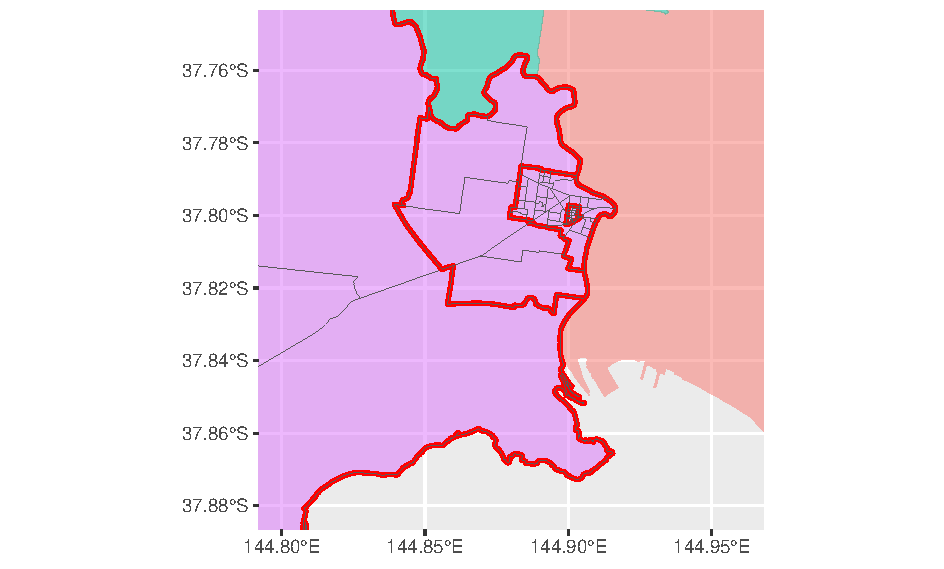
\includegraphics{03-CurrentStudy_files/figure-pdf/fig-FootscraySAexample-1.pdf}

}

\caption{\label{fig-FootscraySAexample}Showing the five SA3 blocks that
make up the `Melbourne - West' SA4 region, the six SA2 blocks that make
up the Maribyrnong SA3 region, the forty SA1 regionsa that make up the
`Footscray' SA2 region, and the sixteen mesh blocks that make up the
central Footscray `21303134811' SA1 region. Note that each red-bounded
area represents a higher resolution (`lower' SA level) than the one that
encloses it. Not Pictured: Boundary of the GMGCCSA.}

\end{figure}

Helpfully, Statistical Areas are also indexed by a structured code
representing their classification hierarchy. For example, SA1 regions
are denoted by an 11 digit code which can be decomposed into the higher
level areas in which the region sits. Figure~\ref{fig-FootscraySA1Code}
demonstrates this for an SA1 region in the area considered above.

\begin{figure}

{\centering 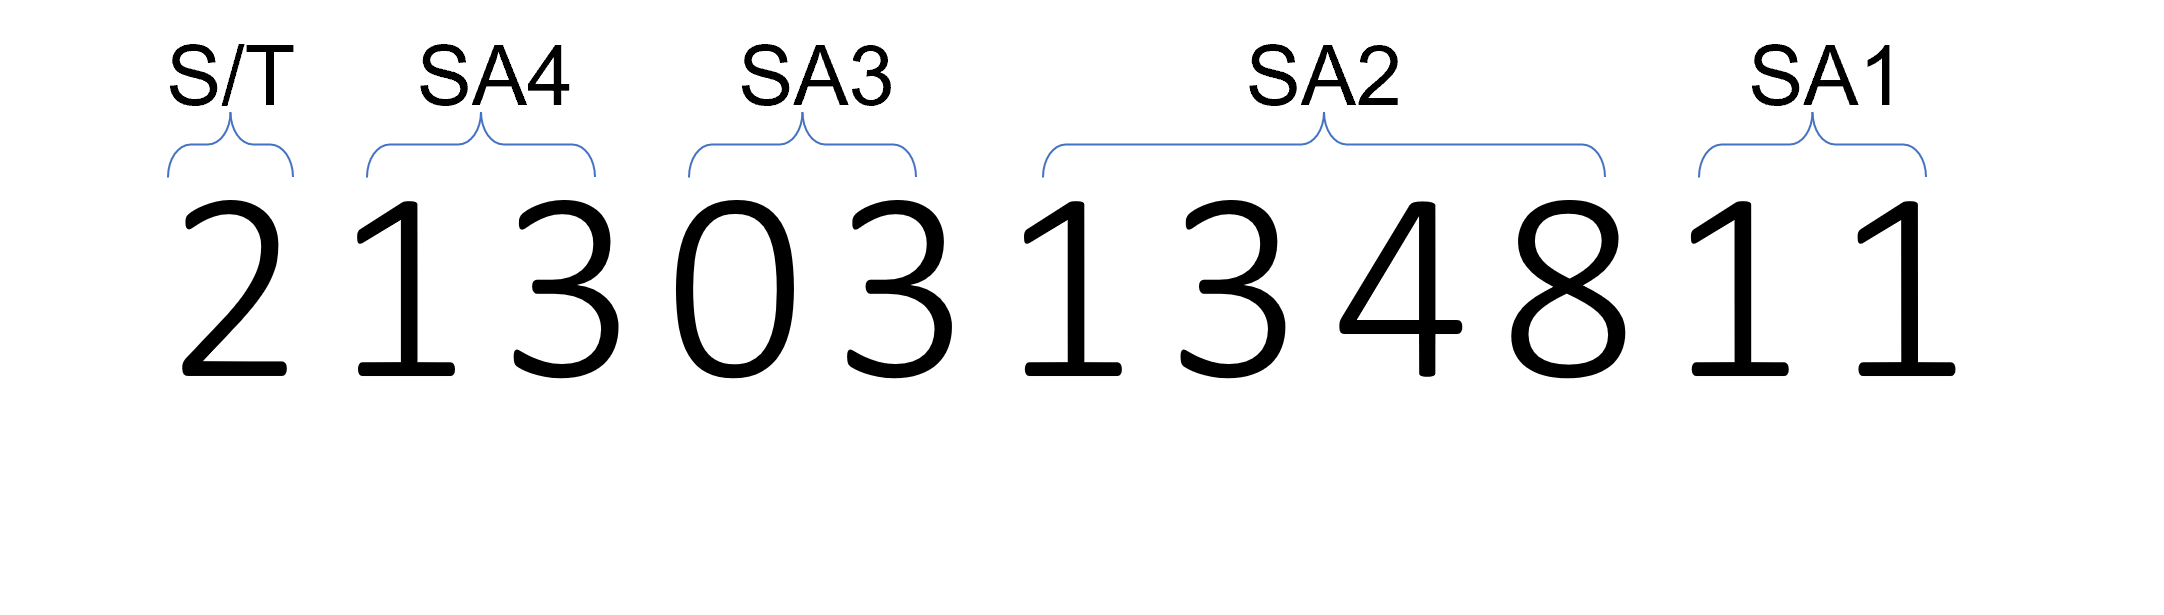
\includegraphics{FootscraySA1eg.png}

}

\caption{\label{fig-FootscraySA1Code}Decomposition of theFootscray SA1
region code from Figure~\ref{fig-FootscraySAexample} into its
hierachical spatial information components}

\end{figure}

\hypertarget{varying-the-spatial-resolution-of-metapopulation-models}{%
\section{Varying the spatial resolution of metapopulation
models}\label{varying-the-spatial-resolution-of-metapopulation-models}}

We can exploit this hierarchical structure by creating meta-population
models incorporating the same overarching spatial structure (i.e.~the
ASGS Statistical Areas structure), but with varying levels of resolution
(e.g.~by using SA2 scale patches instead of SA3 scale patches). Thus, we
can model the GMGCSSA using patches corresponding to different levels of
the SA hierarchy.

\hypertarget{mixing-matrices-to-preserve-homogeneous-mixing}{%
\subsection{Mixing matrices to preserve homogeneous
mixing}\label{mixing-matrices-to-preserve-homogeneous-mixing}}

We might initially consider the models with patch sizes 2, 3, 4 (for
SA2, SA3, SA4), and construct a mixing matrix with uniform mixing across
patches, i.e.~\[
\phi_{ij} = \frac{1}{P_{tot}}
\] Where \(P_{tot}\) is the total number of patches. - How should we
interpret this mixing coefficient? \#\#\# Population proportional mixing

The resulting mixing matrices will be of different sizes (i.e.~40 SA3
patches vs 361 SA2 patches for the Greater Melbourne region), and to
ensure equivalent representation of aggregate levels, patch population
size can be used to scale mixing coefficients, i.e.. for two patches
\(i\) and \(j\) the mixing coefficient \(\phi_{i,j}\):

\[
\phi_{ij} = N_j/N_{tot}
\]

Which gives mixing matrices shown in \textbf{?@fig-GMelbPopMM}

\begin{verbatim}
[[1]]
\end{verbatim}

\begin{verbatim}

[[2]]
\end{verbatim}

\begin{verbatim}

[[3]]
\end{verbatim}

\begin{figure}

{\centering 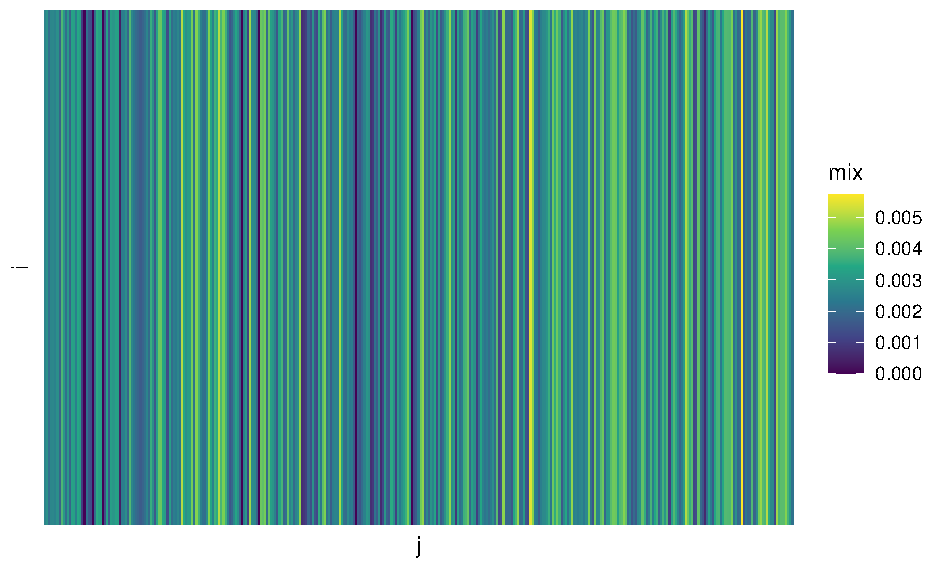
\includegraphics{03-CurrentStudy_files/figure-pdf/fig-GMelbPopMM-1.pdf}

}

\caption{\label{fig-GMelbPopMM-1}\textbf{?(caption)}}

\end{figure}

\begin{figure}

{\centering 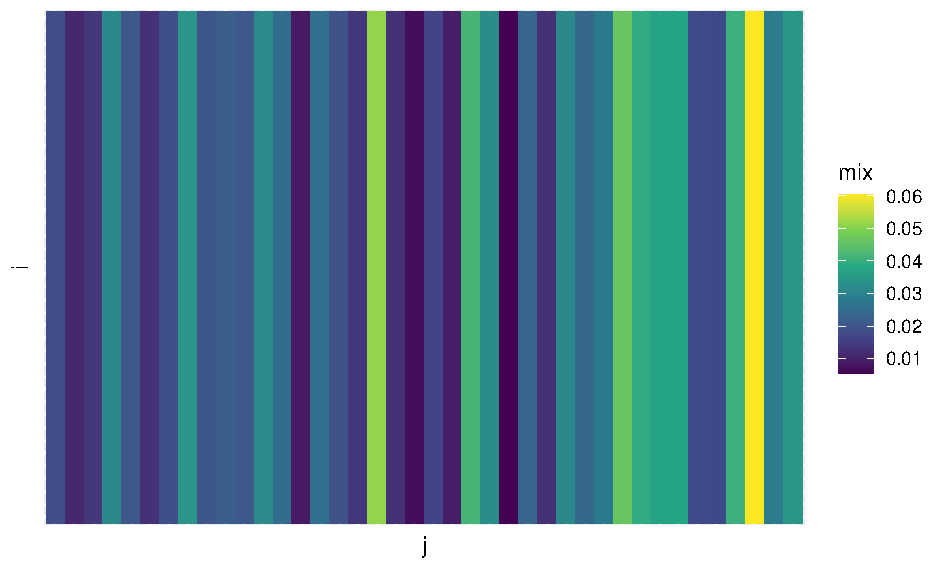
\includegraphics{03-CurrentStudy_files/figure-pdf/fig-GMelbPopMM-2.pdf}

}

\caption{\label{fig-GMelbPopMM-2}\textbf{?(caption)}}

\end{figure}

\begin{figure}

{\centering 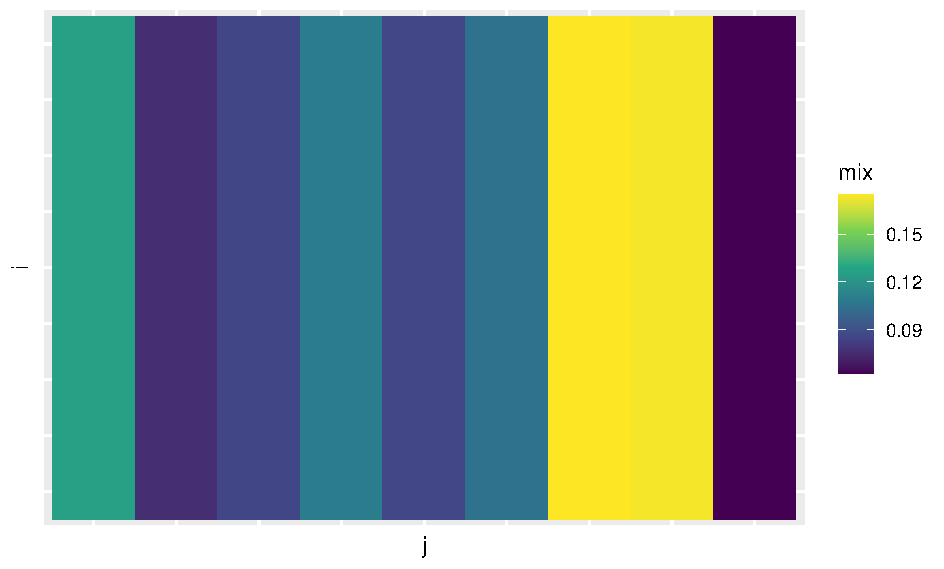
\includegraphics{03-CurrentStudy_files/figure-pdf/fig-GMelbPopMM-3.pdf}

}

\caption{\label{fig-GMelbPopMM-3}\textbf{?(caption)}}

\end{figure}

We can implement a metapopulation model using these mixing matrices as
described in chapter Chapter~\ref{sec-MPMspec}, to briefly summarise:

\hypertarget{results-equivalent-models-at-different-spatial-resolution}{%
\paragraph{Results: equivalent models at different spatial
resolution}\label{results-equivalent-models-at-different-spatial-resolution}}

-total size -peak size -Duration of pop prop models with SA2 SA3 SA4
homogeneous patches - Expect equivalence

\hypertarget{statistical-area-mixing-structure}{%
\subsubsection{Statistical Area Mixing
structure}\label{statistical-area-mixing-structure}}

We can also enforce heterogenous mixing, while simultaneously encoding
the hierarchical structure of the SA classification by constructing
hierarchical block mixing matrices. To do so, we specify a set of
coefficients \(\xi = [\xi_1, ..., \xi_i]\) which determine the
proportion of mixing occurs at each level of the spatial hierarchy. Note
that \[
\sum\limits_{i}\xi=1
\] This coefficient is distributed amongst patches occurring in the same
level \(L\) region, so mixing for any two patches, \(i\) and \(j\) \[
M_{ij}= \frac{\xi_{L}}{N^{L}} 
\] if \[
j \in S_{i}^{L}
\] but \[j \notin S_{i}^{L-1}\] Where \(S_{i}^{L}\) is the set of
patches in the same level \(L\) region as \(i\).

To extend the example from \textbf{?@sec-XX}, we can consider a subset
of SA2 regions from the GMGCCSA ((\textbf{tab-MMeg?}))

\begin{figure}

{\centering 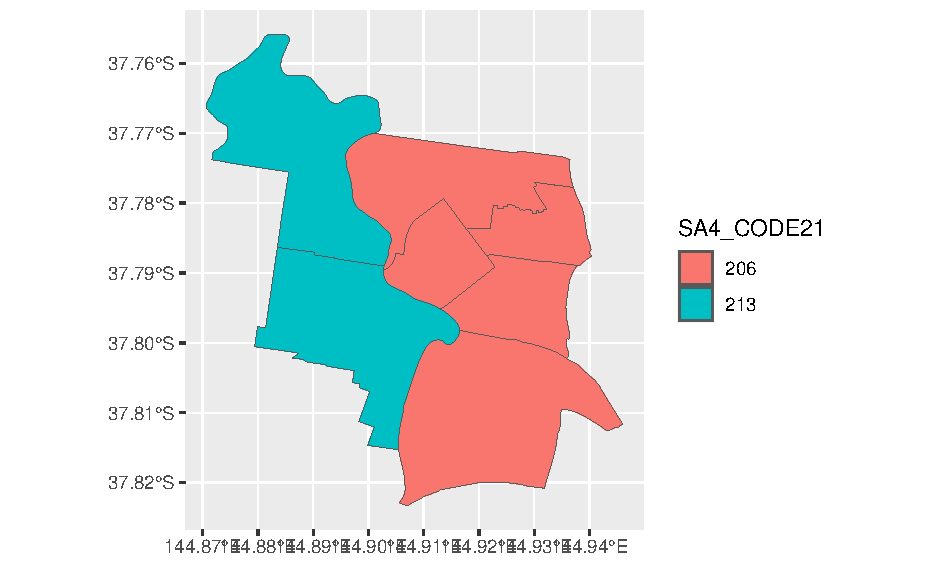
\includegraphics{03-CurrentStudy_files/figure-pdf/fig-Example_region-1.pdf}

}

\caption{\label{fig-Example_region}\textbf{?(caption)}}

\end{figure}

Kensington, Racecourse, and West industrial are SA2 regions within the
`Melbourne City' SA3 region, Footscray and Maribyrnong are SA2 regions
within the `Maribyrnong' SA3 region, and Flemington and Ascot Vale are
SA2 regions withing the `Essendon' SA3 region. Furthermore, both
`Melbnourne city' and Essendon are within the `Inner Melbourne' SA4
region while Marybyrnong lies iside the `West Melbourne' SA4 Region

To model these SA2 patches in isolation, we can construct a
\(7 \times 7\) mixing matrix, row by row, for
\(\xi = \left[ \frac{1}{4}, \frac{1}{4},\frac{1}{4},\frac{1}{4} \right]\)as
follows:

let \(i =\) \texttt{Kensington}. Since \texttt{Kensington} is it's own
SA2 region, \[M_{i,i} = \frac{1}{4}\]When \(j\) is a region in
\texttt{Melbourne\ City} SA3 (alongside \texttt{Kensington}), like
\texttt{West\ Industrial} or \texttt{Racecourse}, \(M_{i,j}\) will be a
proportion of \(\xi_{SA3}\). For \(j = Racecourse\) and
\(j = West Industrial\) \[
M_{i,j} = \frac{\xi_{SA3}}{N_{i}^{SA3} - N_{i}^{SA2}} = \frac{\frac{1}{4}}{3 - 1} = \frac{1}{8}
\] When patch \(j\) occurs outside the Melbourne City SA3, but within
the \texttt{Inner\ Melbourne} SA4, like those in \texttt{Essendon}SA3 \[
M_{i,j} = \frac{\xi_{SA4}}{N_{i}^{SA4} - N_{i}^{SA3}} = \frac{\frac{1}{4}}{5 - 3} = \frac{1}{8}
\] Finally when \(j\) is a patch outside the \texttt{Inner\ Melbourne}
SA4, like those in \texttt{West\ Melbourne}SA4 \[
M_{i,j} = \frac{\xi_{SA5}}{N_{i}^{SA5} - N_{i}^{SA4}} = \frac{\frac{1}{4}}{7 - 3} = \frac{1}{16}
\] thus for the row \(M_{i}\), representing the mixing of individuals
from Kensington, \$ sum\limits*\{j\}M*\{j\}= \frac{1}{4} +\frac{1}{8} +
\frac{1}{8} +\frac{1}{8} + \frac{1}{8} + \frac{1}{8} + \frac{1}{8} = 1\$
as desired. Repeating this for all patches \(i\), gives the mixing
matrix represented in Figure~\ref{fig-egMM}

\begin{figure}

{\centering 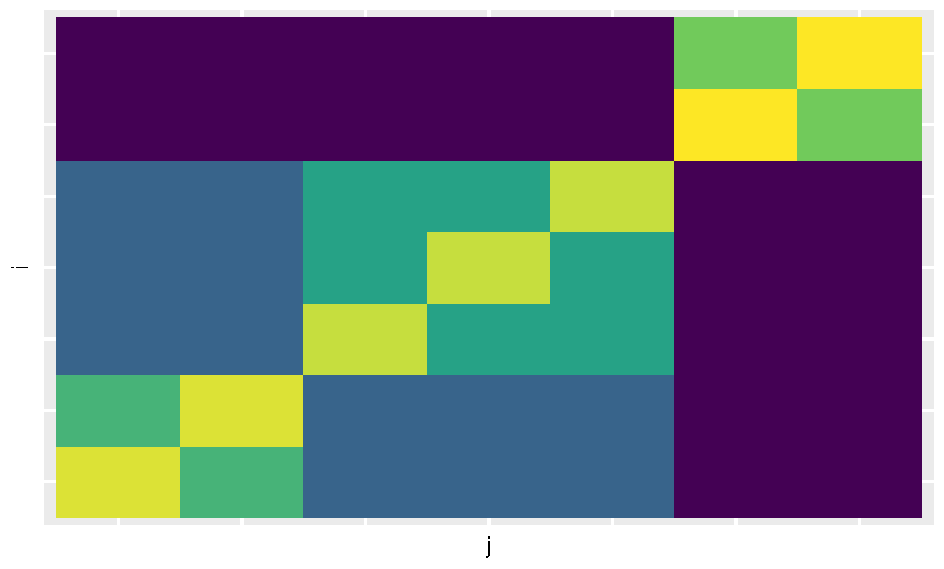
\includegraphics{03-CurrentStudy_files/figure-pdf/fig-egMM-1.pdf}

}

\caption{\label{fig-egMM}\textbf{?(caption)}}

\end{figure}

Applying this process to the whole GMGCCSA yields the mixing matrices
presented in figure \textbf{?@fig-GCC\_HMM}

\begin{verbatim}
$SA2
\end{verbatim}

\begin{verbatim}

$SA3
\end{verbatim}

\begin{verbatim}

$SA4
\end{verbatim}

\begin{figure}

{\centering 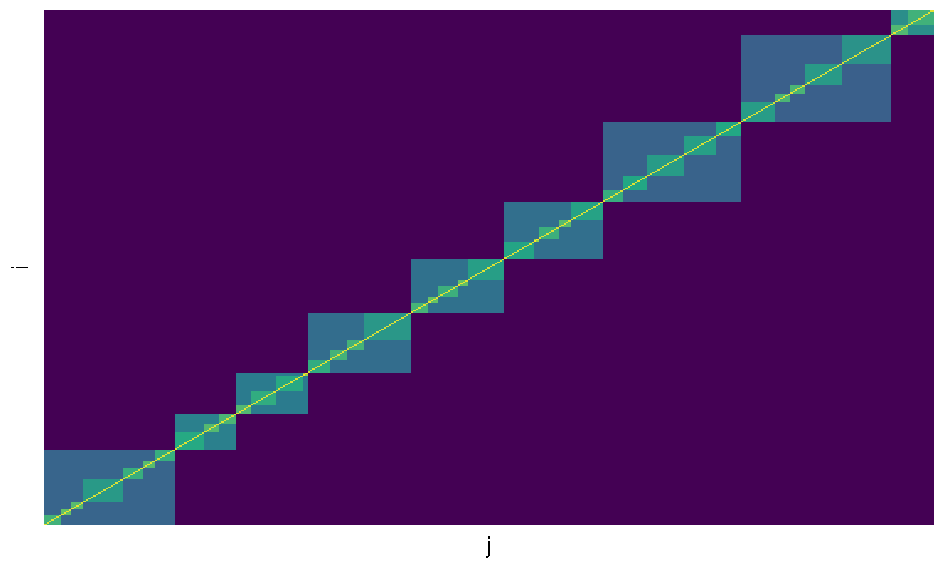
\includegraphics{03-CurrentStudy_files/figure-pdf/fig-GCC_HMM-1.pdf}

}

\caption{\label{fig-GCC_HMM-1}\textbf{?(caption)}}

\end{figure}

\begin{figure}

{\centering 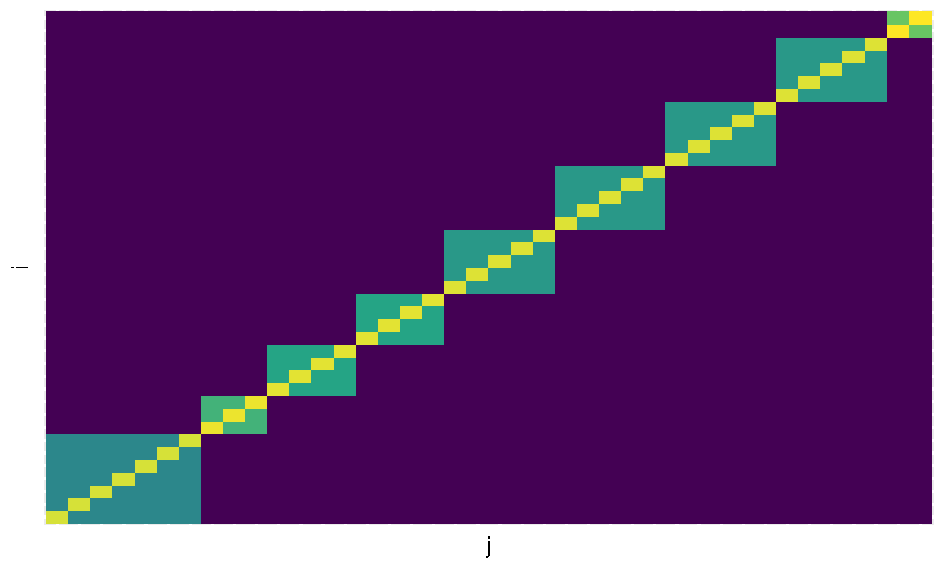
\includegraphics{03-CurrentStudy_files/figure-pdf/fig-GCC_HMM-2.pdf}

}

\caption{\label{fig-GCC_HMM-2}\textbf{?(caption)}}

\end{figure}

\begin{figure}

{\centering 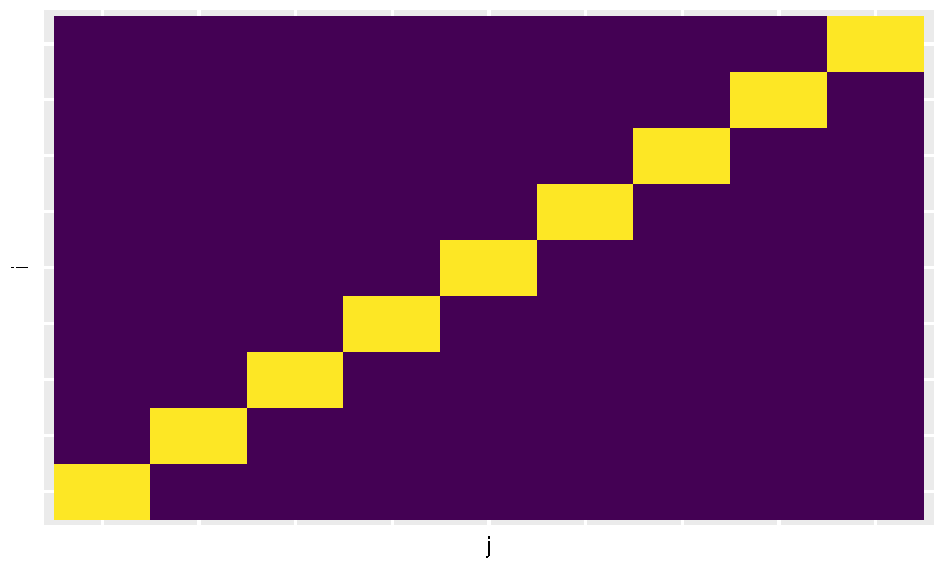
\includegraphics{03-CurrentStudy_files/figure-pdf/fig-GCC_HMM-3.pdf}

}

\caption{\label{fig-GCC_HMM-3}\textbf{?(caption)}}

\end{figure}

\bookmarksetup{startatroot}

\hypertarget{chapter-4.-modelling-intervention}{%
\chapter{Chapter 4. Modelling
intervention}\label{chapter-4.-modelling-intervention}}

\bookmarksetup{startatroot}

\hypertarget{bibliography}{%
\chapter*{Bibliography}\label{bibliography}}
\addcontentsline{toc}{chapter}{Bibliography}

\markboth{Bibliography}{Bibliography}

\hypertarget{refs}{}
\begin{CSLReferences}{1}{0}
\leavevmode\vadjust pre{\hypertarget{ref-2023AustralianStatisticalGeographya}{}}%
Australian statistical geography standard (ASGS), (2023).

\leavevmode\vadjust pre{\hypertarget{ref-renv}{}}%
Ushey, K. (2022). \emph{{renv}: Project environments}.
\url{https://CRAN.R-project.org/package=renv} R package version 0.16.0

\end{CSLReferences}

\cleardoublepage
\phantomsection
\addcontentsline{toc}{part}{Appendices}
\appendix

\hypertarget{additional-stuff}{%
\chapter{Additional stuff}\label{additional-stuff}}

You might put some computer output here, or maybe additional tables. It
is possible to have multiple appendices. Just list them in the
appropriate place within \texttt{\_quarto.yml}.



\end{document}
